\documentclass[a4paper,11pt]{report}
\usepackage[utf8]{inputenc} % UTF8 юникод текст оруулах

\usepackage[T2A]{fontenc} % кирил үсгийн кодчилол
\usepackage[mongolian]{babel} % олон хэлний текст
\usepackage{pdfpages}
\usepackage{graphicx} % зураг оруулах
\usepackage{epstopdf}
\usepackage{latexsym}
\usepackage{rotating} % эргүүлэх
\usepackage{fancybox} % хүрээлэх
\usepackage{amsmath} % гоё математикийн тэмдэг
\usepackage{bm} % дармал математик
\usepackage{color} % өнгөөр бичих
\usepackage{fancyhdr} % хуудасны хөл, толгой
%\usepackage[backend=biber, url=true, natbib=true]{biblatex}
\usepackage{hyperref}
\hypersetup{colorlinks=true}
\usepackage{multirow}
%\bibliographystyle{plain}
%\bibliography{ref.bib}
%\addbibresource{ref.bib}
\bibliographystyle{abbrv}

\usepackage{pgf}
\usepackage{tikz} % зураг зурах
\usetikzlibrary{arrows,automata}

\usepackage{thesis} % ШУТИС -ийн тезисийн формат

\pagestyle{fancy}


\usepackage{listings}
\usepackage{color}
 
\definecolor{codegreen}{rgb}{0,0.6,0}
\definecolor{codegray}{rgb}{0.5,0.5,0.5}
\definecolor{codepurple}{rgb}{0.58,0,0.82}
\definecolor{backcolour}{rgb}{0.95,0.95,0.92}
 
\lstdefinestyle{mystyle}{
    backgroundcolor=\color{backcolour},   
    commentstyle=\color{codegreen},
    keywordstyle=\color{magenta},
    numberstyle=\tiny\color{codegray},
    stringstyle=\color{codepurple},
    basicstyle=\footnotesize,
    breakatwhitespace=false,         
    breaklines=true,                 
    captionpos=b,                    
    keepspaces=true,                 
    numbers=left,                    
    numbersep=5pt,                  
    showspaces=false,                
    showstringspaces=false,
    showtabs=false,                  
    tabsize=2    
}

\lstset{
	language=php, %% Troque para PHP, C, Java, etc... bash é o padrão
	basicstyle=\ttfamily\small,
	numberstyle=\footnotesize, 
	numbers=left,
	    backgroundcolor=\color{backcolour},   
    commentstyle=\color{codegreen},
    keywordstyle=\color{magenta},
    numberstyle=\tiny\color{codegray},
    stringstyle=\color{codepurple},
	frame=single,
	tabsize=2,
	rulecolor=\color{black!30},
	title=\lstname,
	escapeinside={\%*}{*)},
	breaklines=true,
	breakatwhitespace=true,
	framextopmargin=2pt,
	framexbottommargin=2pt,
	extendedchars=false,
	inputencoding=utf8
}
%\lstset{style=mystyle}

\usepackage{url} % hyperref works too
\urlstyle{same}


\lstset{language=C++,texcl=true}

\begin{document}

\pagenumbering{roman}

% Гарчиг, зохиогч, горилсон зэрэг, тэнхим/багийн нэр болон он сарыг оруулах.
% Оруулсны дараах байдал:
%\thesistitle
%	{Диссертаци/тезисийн нэр}
%	{Зохиогчийн нэр}
%	{Горилсон зэрэг}
%	{Тэнхим/багийн нэр}
%	{Огноо}
%\thesistitle командын тодорхойлолт thesis.sty -д байгаа бөгөөд
% өөр бусад тохиргоог энд хийж болно.

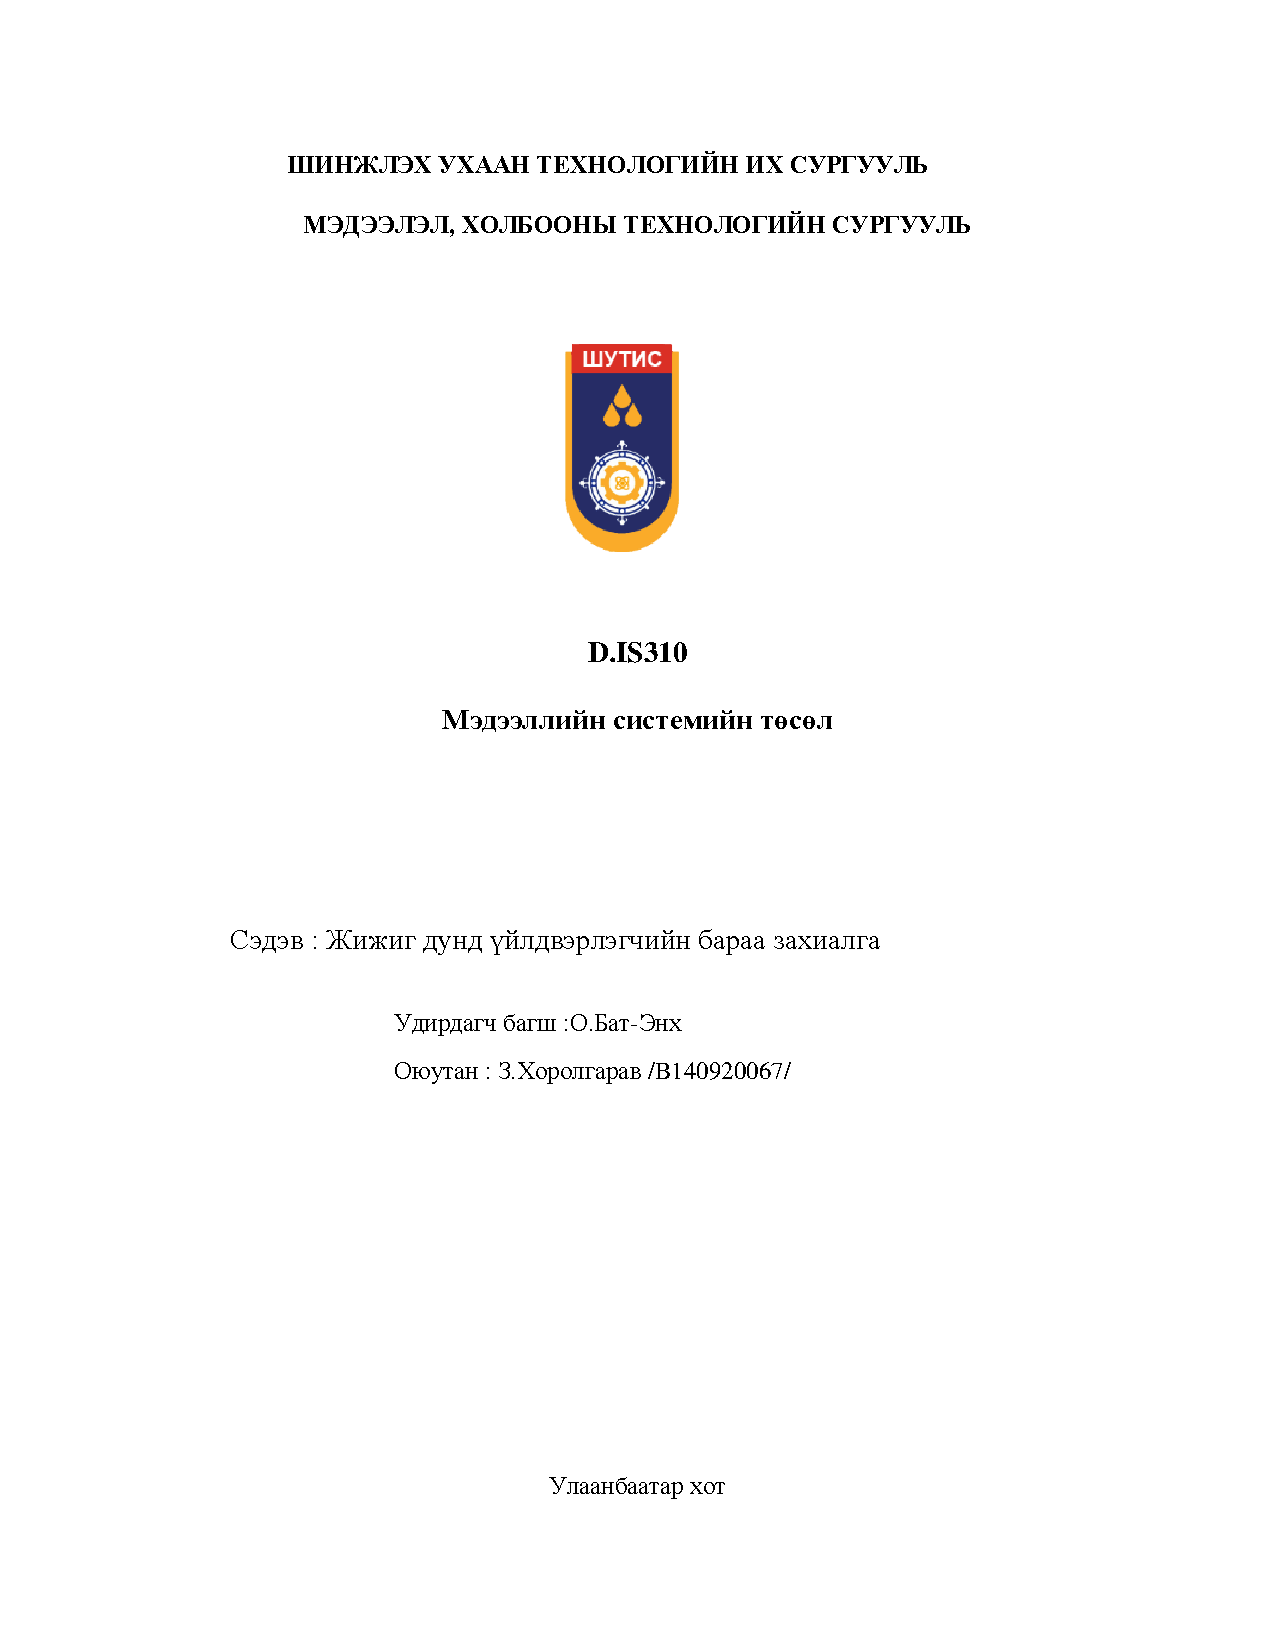
\includepdf[page={1}]{Nvvr.pdf}
%
\includepdf[page={1-5,9,11,15,19,23,24,29,30,32,34,35-54}]{last.pdf}
%
\includepdf[page={6-8,10,12-14,16-18,20-22,25-28,31,33}]{last.pdf}
\include{abstract}
\tableofcontents

\include{tables}
\addcontentsline{toc}{chapter}{Зургийн жагсаалт}
\listoffigures



\include{bib}

\pagenumbering{arabic}
\chapter{1.	Удиртгал }
\label{chap:intro}
\section{Зорилго}
•  Eschool-ийн Зураг засварлагч системийн гол зорилго нь зураг харна,илгээх,устгана,текст бичих байршуулах зэргийг ашиглаж зураг засвар хийхэд оршино.


\section{Зорилт} 


Энэхүү төслийн нэн тэргүүний зорилт нь:

\begin{itemize}
	
	\item Системд үйлчилгээний аюулгүй байдлыг бүрэн хангасан, хэрэглэгчдийн мэдээллийн нууцлалыг хариуцан ажиллах веб сайт хийх
	
	\item Үйлдвэрлэгчийн бүтээгдэхүүний танилцуулга тодорхой байх
	
	\item Хэрэглэгчийн үйл ажиллагааг хөнгөвчлөх
	
\end{itemize}




\section{Системийн хамрах хүрээ }
eschool системийг ашиглаж байгаа хэрэглэгч ашиглана. 

\chapter{2.	Судалгааны хэсэг}
\label{chap:intro}
\section{Хэрэглэгчийн судалгааны хэсэг}
\textbf{фотошоп програм гэж юу вэ?}
фотошоп програм програм нь растерийн дүрслэлийг бүтээдэг. PHOTOSHOP програмд дээр ажиллаж байгаа хамгийн том дүрслэлдийн тоо 30000х30000 рiхel цэгийн харьцаатай хамгийн өндөр нягтрал нь 10000dpi байдаг Файлын хамгийн том хэмжээ нь 2GB байдаг.
Уг програм дээр ажилладаг мэргэжилтэн нь дэлгэцэнд өөрийн дүрслэн бодсоноороо ямар ч зохиомжийг зурж байгуулж болох ба түүний хувилбаруудыг хадгалах тэднийг сканнердсан дүрслэлтэй нь хослуулан зохицуулах нийлүүлэх , дүрсний шилжилт, зөөлт болон фильтрийн олон аргуудыг хэрэглэдэг.
PhotoShop програмаар шинээр шинэ файл үүсгэхэд энэ нь нэг цэг дээр олон өнгийг олгох чадвартай давхаргатай зураг үүсгэдэг. Ийм учраас энэхүү програмд зургийн файлтай ажиллаж байх үед хийгдэж байгаа өөрчлөлт нь зөвхөн идэвхтэй давхаргын хувьд хийгддэг.

\end{itemize}

\chapter{Төслийн хэсэг}
\label{chap:intro}
\section{Системийн хэрэглэгчид}
\begin{itemize}
	\item  хэрэглэгч
	\item  Админ
\end{itemize}
\section{Функционал шаардлага}
\begin{itemize}
	\item  хэрэглэгч
	\item  Админ
\end{itemize}
\begin{itemize}
	\item [1]Зураг Засах
	\item [1.1] Зураг тодоруулна
	\item [1.2] Зурагийн хэмжээ ихэсгэнэ
	\item [1.3] Зурагийн хэмжээ багасгана
	\item [1.4] Эргүүлнэ
	\item [1.5] Тайрах
	\item [1.6]текст бичих
	\item [1.7]Байршуулах
	\item [2] Зураг харна
	\item [3]Илгээх
	\item [4]Устгана
	\item [5]Хариу үйлдэл үзүүлэх(Сэтгэл хөдлөл)
	\begin{itemize}
		\item [1]Бүртгэх
		\item [2]Нэмэх
		\item [3]Хасах
	\end{itemize}
	\section{Функционал бус шаардлага}
	\begin{itemize}
		\item Засах мэдээллийг 5 секундэд хийдэг байх
		\item Системийн загвар хүнд ойлгомжтой байх
		\item Системийг тестэлж, хамгаалсан байх
\end{itemize}
\newpage
\section{ Юз кейс диаграм , түүний тодорхойлолт }

\subsection{Юз кейз  диаграм} 
Энэ диаграм нь ямар функцуудыг гүйцэтгэх, хэтийн төлөв, хэрэгцээ шаардлагуудаас системийг дүрслэн харуулна. 

\munepsfig[width=\textwidth, height=12cm]{Use Case.jpg}{ Юзкейс диаграм }
\newpage

\subsection{ Юз кейз тодорхойлолт }
\begin{center}
	\begin{table}[!htbp]
		\caption{Зураг засах юзкейс диаграмын тодорхойлот}
		\begin{tabular}{|p{4cm}|p{11cm}|}
			\hline
			Товч тайлбар: &Зургийг будах, зураг багагсгах гэх мэт өөр хэрэгтэй байдлаар зургийг өөрчлөх \\
			\hline
			Триггер: & Бүтээгдэхүүн захиалгын модулиудыг ашиглахын тулд системд нэвтрэх шаардлагатай болсон. \\
			\hline
			Үндсэн оролцогч: &  хэрэглэгч \\
			\hline
			Нэмэлт оролцогч: & Байхгүй \\
			\hline
			Өмнөх нөхцөл: &  Зураг засахын өмнө зургийг оруулсан байна\\
			\hline
			Ажлын урсгал: & \begin{enumerate}
				\item Зургийн хэсэгрүү орно.
				\item	Хэрэгсэлүүд ашиглан зургийг өөрт хэрэгтэй байдлаар засварлана
				
			\end{enumerate}
				\\		 
			 \hline
			Дараах нөхцөл: & 	Зураг засагдсан байна.. 	\\	
		   
		  \hline	Альтернатив урсгал: & 	Байхгүй	 
			
			\\	\hline
		\end{tabular}
	\end{table}
\end{center}


\begin{center}
	\begin{table}[!htbp]
		\caption{Зураг илгээх Юзкейз тодорхойлолт}
		\begin{tabular}{|p{4cm}|p{11cm}|}
			\hline
			Нэр: & Зураг илгээх \\
			\hline
			ID: &2\\
			\hline
			Товч тайлбар: &Сошиал дахь найзтайгаа зураг хуваалцахыг хүссэн үед зураг илгээх \\
			\hline
			Триггер: & Системд бүртгэгдээгүй шинэ барааг бүртгэлтэй болгох \\
			\hline
			Үндсэн тоглогч: & хэрэглэгч \\
			\hline
			Нэмэлт тоглогч: & Бусад хэрэглэгч \\
			\hline
			
			Өмнөх нөхцөл: & \begin{enumerate}
				\item Зураг веб-д эсхүл өөрийн компьютерт байна.
			\end{enumerate}	\\
			\hline
			Үндсэн урсгал: & 
			
			\item Зургийн хэсэгрүү орно.
			\item Зургийг илгээх товч дарна.
			\item Зураг илгээх хүнээ сонгоно
			\item Зургаа илгээнэ.
				
			\\		 
			\hline
			Дараах нөхцөл: & Зураг илгээгдсэн байна 	\\	
			
			\hline	Альтернатив урсгал: & Байхгүй 	\\
			\hline
		\end{tabular}
	\end{table}
\end{center}

\begin{center}
	\begin{table}[!htbp]
		\caption{Хариу үйлдэл үзүүлэх (Сэтгэл хөдлөл) Юзкейз тодорхойлолт}
		\begin{tabular}{|p{4cm}|p{11cm}|}
			\hline
			Нэр: & Хариу үйлдэл үзүүлэх (Сэтгэл хөдлөл) \\
			\hline
			ID: &3 \\
			\hline
			Товч тайлбар: &Өөрт таалагдсан болон таалагдаагүй зураг нь дээрээ хариу үйлдэл үзүүлэх \\
			\hline
			Триггер: & Байхгүй \\
			\hline
			Үндсэн тоглогч: & Хэрэглэгч \\
			\hline
			Нэмэлт тоглогч: & Байхгүй \\
			\hline
			
			Өмнөх нөхцөл: & \begin{enumerate}
				\item Зураг системд байршсан байх  
			\end{enumerate}	\\
			\hline
			Үндсэн урсгал: & 
			\item Зургийг үзнэ
			\item Хариу үйлдэл үзүүлнэ..
			
			\\		 
			\hline
			Дараах нөхцөл: & Зураг хариу үйлдэлтэй болно. 	\\	
			\hline	Альтернатив урсгал: & Байхгүй 	\\
			\hline
		\end{tabular}
	\end{table}
\end{center}

\newpage
\section{Ашигласан технологийн шаардлага}

\subsection{Програм ажиллах үйлдлийн системийн сонголт:}

\begin{itemize}
	\item Windows OS: 2007,2008,2010
\end{itemize}

Хамгийн өргөн хэрэглэгддэг нь Microsoft corporation-ийн windows үйлдлийн систем юм.  Windows үйлдлийн системийн давуу талууд :

\begin{itemize}
	\item Хэрэглэхэд хялбар
	\item Асалт илүү хурдан
	\item Бусад техник төхөөрөмжүүдтэй хамгийн сайн зохицдог
	\item Цэнэг (батерей) барилт удаан
	\item Нягтралттай бүхий л дэлгэцэнд тохирох
	\item Windows-ийн бүхий л дагалдах хэрэгсэлтэй холбогдох боломжтой
\end{itemize}

\subsection{Програм хөгжүүлэх хэлний сонголт:}

PHP  програмчлалын хэлийг ашиглан системээ хөгжүүлнэ. PHP програмчлалын хэл нь: 

\begin{itemize}
	\item Сервер талын скрипт хэл
	\item Бүхий л төрлийн үйлдлийн систем/windows, macintosh…/ сервер / Apach, ISS…/ өгөгдлийн сан /MySQL, Oracle, MsSQL, Access…/ дээр ажилладаг.
	\item Сервер дээр файлуудыг нээх, хаах, унших, бичих гэх мэт файлтай ажиллах бүх үйлдлүүдийг хийнэ. 
	\item Хүссэн хуудсандаа хэрэглэгчийн хязгаарлалт хийх боломжтой
	\item Өгөгдлийг хүссэнээрээ нууцалж, кодолж чаддаг
	\item Өгөгдлийн санг үүсгэх, устгах, өгөгдөл нэмэх, устгах, засварлах, хайх гэх мэт үйлдлүүдийг хийдэг
	\item Session, cookie хувьсагчтай ажилладаг
	\item Үнэгүй нээлттэй эх
	\item Динамик веб сайт хийхэд тохиромжтой юм. 
\end{itemize}

\subsection{Өгөгдлийн сангийн удирдах системийн сонголт:}

MySQL өгөгдлийн сан удирдах системийг сонгосон. MySQLнь: 

\begin{itemize}
	\item MySQL нь хамгийн их өргөн тархсан нээлттэй эх код бөгөөд SQL өгөгдлийн сангийн удирдах систем юм. Хүссэн хүн интернэтээс үнэгүй татаж, ашиглах боломжтой. 
	\item Хурдан, найдвартай, ашиглахад хялбар
	\item Их хэмжээний өгөгдөлтэй ажиллах боломжтой/ойролцоогоор 60000 хүснэгт, 50 сая бичлэг/ 
	\item Платформоос үл хамаарч ажиллаж чаддаг бөгөөд бүх платформ дээр ижил үр дүнтэйгээр ажилладаг.
	\item Нээлттэй эх код систем учраас дэлхийн олон мянган мэргэжилтэн хөгжүүлэгч нар алдааг засварлаж, хөгжүүлж байдаг.
	\item C, C++, Eiffel, Java, Perl, PHP, Python, Ruby зэрэг хэлүүдэд зориулан API гаргасан байдаг. Програмчлалын хэлнүүдтэй холбохын тулд ашигладаг Connector/ODBC, Connector/ J, Connector/NET зэрэг холбогчуудыг хувилбар болгон өөр дээрээ гаргадаг. 
	\item Интернэт сүлжээгээр өгөгдлийн санд хандахад холболт, хурд, нууцлалыг тусгаж өгсөн
	\item Олон хэлний горимыг дэмждэг. Алдааны мэдээлэл зэргийг хүссэн хэлээрээ гаргах боломжтой. Өгөгдлөө unicode2-оор хадгалахаас гадна эрэмбэлж болдог. 
\end{itemize}

\subsection{Баримт бичгийн боловсруулалтын системийн сонголт}

Бичиг баримт боловсруулалттай ажлын хувьд:

\begin{itemize}
	\item MS Office Word 2016 
	\item Visual Paradigm for UML 14.1
	\item Enterprise Architecture 
\end{itemize}

Танилцуулах програмын хувьд:

\begin{itemize}
	\item MS Office PowerPoint 2016. 
\end{itemize}




\chapter{Өгөгдлийн сангийн зохиомж}
\label{chap:intro}
\section{Өгөгдлийн ерөнхий схем }

\munepsfig[width=\textwidth, height=6cm ]{erd.jpg}{Өгөгдлийн ерөнхий схемийн диаграм}

\newpage

\chapter{Системийн зохиомж}
\label{chap:intro}
\section{Дэлгэцийн зохиомж}

\munepsfig[width=\textwidth,height=12cm ]{Delgets.jpg}{Хэрэглэгчийн нүүр хуудас }

\pagebreak

\section{Класс диаграм (class diagram)}
\munepsfig[width=\textwidth,height=15cm ]{entityClass.jpg}{ Класс диаграм }
\munepsfig[width=\textwidth,height=15cm ]{boundaryClass.jpg}{ Класс диаграм }
\munepsfig[width=\textwidth,height=15cm ]{controlClass.jpg}{ Класс диаграм }
\munepsfig[width=\textwidth,height=15cm ]{finalClass.jpg}{ Класс диаграм }
\pagebreak

\section{Үйл ажиллагааны диаграм (Activity Diagram) }

\munepsfig[width=\textwidth,height=12cm ]{Activity.jpg}{ Хэрэглэгч зураг засах үйл ажиллагааны диаграм }


\pagebreak

\section{Дарааллын диаграм (Sequence diagram)}
Энэ диаграм нь системийн объектууд хоорондоо хэрхэн харилцдагийг дараалласан зурвас байдлаар тодорхойлох ба энэ зурвасуудад харгалзах объектуудын амьдрах хугацааг үзүүлдэг.

\munepsfig[width=\textwidth,height=12cm ]{Sequence Diagram1.jpg}{зураг засах дарааллын диаграм }



\pagebreak

\section{Төлөв шилжилтийн диаграм (State diagram)}

\munepsfig[width=\textwidth,height=12cm ]{State.jpg}{ Засахын төлвийн диаграм }

\pagebreak



\end{itemize}











\chapter{Дүгнэлт}
\label{chap:intro}
\paragraph{}
Манай энэхүү ажлын хүрээнд зураг завсарлагч системийн web application хувилбарыг хэрэгжүүлсэн ба PHP хэл дээр MySQL өгөгдөлийн сан ашиглан бүтэээлээ. Eschool-ийн Зураг засварлагч системийн гол зорилго нь зураг харна,илгээх,устгана,текст бичих байршуулах зэргийг ашиглаж зураг засвар хийж байгаа..

\begin{thebibliography}{9}

\bibitem{rasp} Ц. Ганбат “Хүн ба компьютерийн харилцаа” 2009	
 
\bibitem{pythn} Б.Батзолбоо ‘UML 2.0 Объект хандлагат шинжилгээ ба түүний хэрэглээ’ 2015

\end{thebibliography}




%\include{bib1}


% Хэрэв хавсралт байхгүй бол дараах мөрүүдийг хасаж болно.
% Олон хавсралттай бол нэмэж болно.
%\appendix

%chapter{Юунаас эхлэх вэ?}
\label{apdx:B}
Мэдээж \LaTeX{} системийг өөрийн компьютерт суулгах хэрэгтэй. Үүний тулд:
\begin{itemize}
	\item \LaTeX татан авч суулгах. MikTex, TeX Live гээд олон янзын хувилбар бий. Windows системд хамгийн тохиромжтой нь MikTex: \url{http://www.miktex.org}
	\item \LaTeX{} -тай ажиллах орчинг татан авч суулгах. Ер нь дурын редактор болно. Гэхдээ зориулалтынх байвал илүү тохиромжтой(\url{http://en.wikipedia.org/wiki/Comparison_of_TeX_editors}). Үнэтэй системээс WinEdt: \url{http://www.winedt.com}, Үнэгүйгээс TeXstudio: \url{http://texstudio.sourceforge.net} -г илүүд үздэг.
	\item Монголоор алдаагүй бичихэд ''Open Office'' толь: \url{http://wiki.openoffice.org/wiki/Dictionaries} хэрэг болно.
	\item \LaTeX{} -ийн гарын авлага (интернетээр дүүрэн). Эхэлж үзэх сонгодог материал бол ''The Not So Short Introduction to \LaTeXe. Маш олон хэл дээр хөрвүүлэгдсэн. Түүний дотор Монгол: \url{http://www.ctan.org/tex-archive/info/lshort}. Мөн Wikibook: \url{http://en.wikibooks.org/wiki/LaTeX}
	\item \LaTeX{} сонирхогчдыг татдаг булан: \url{http://www.tug.org/begin.html}, сонирхолтой жишээ: \url{http://www.texample.net/tikz/}
	\item Бэлэн загвар: \url{http://www.latextemplates.com/}
	 
\end{itemize}



\end{document}
